\section{OpenQuake Hazard: main concepts}
The OpenQuake-Hazard module offers the capability to perform seismic hazard analysis (SHA) following various approaches. Currently three main types of analysis are supported:
\begin{itemize}
\item \textbf{Classical probabilistic SHA}, allowing calculation of hazard curves and hazard maps  following classical integration procedure (\cite{cornell1968}) as formulated by \cite{field2003}.
\item \textbf{Event-Based probabilistic SHA}, allowing calculation of ground motion fields from stochastic event sets.
\item \textbf{Deterministic SHA}, allowing calculation of ground motion field realizations from single  earthquake rupture scenario.
\end{itemize}
Each type of analysis involve a number of calculators, each responsible for a specific task.
\begin{figure}[htbp]
\begin{center}
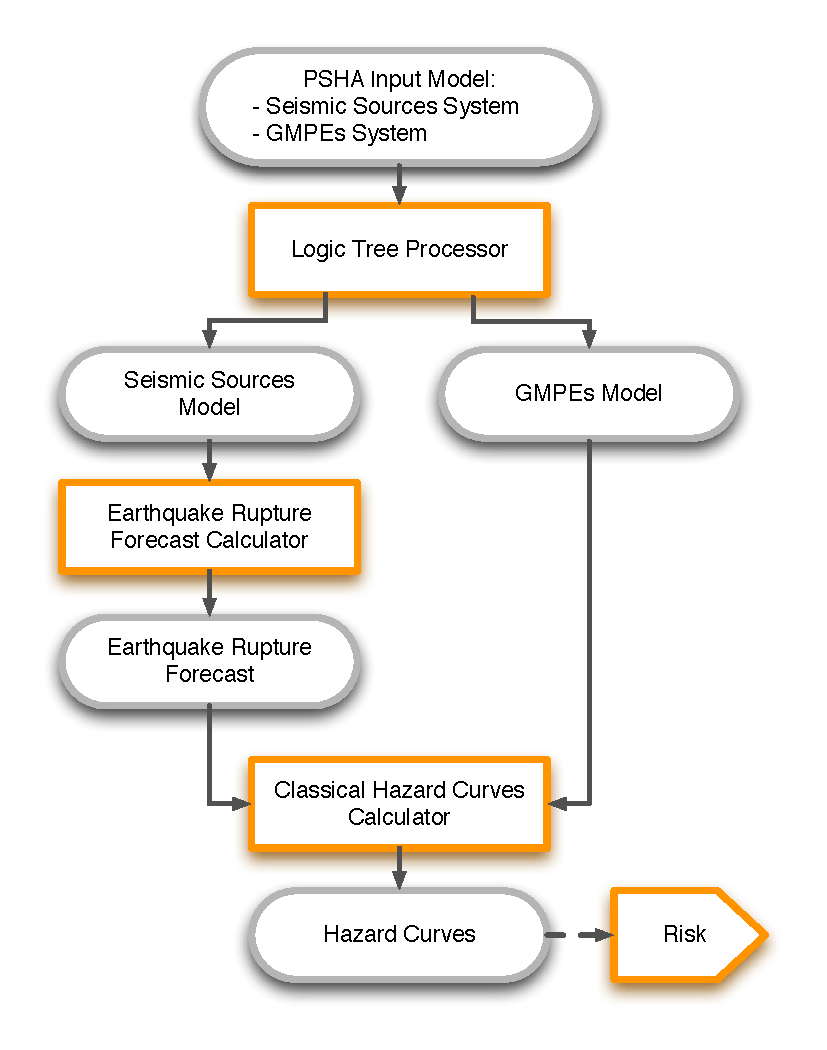
\includegraphics[width=10cm]{./Figures/Part_Hazard/classical_psha_workflow.eps}
\caption{Workflow for classical PSHA. Given a seismic hazard model (expressed as source model and GMPE logic trees), the Logic Tree Processor is responsible for selecting a particular source model and GMPE. The source model is then provided to the Earthquake Rupture Forecast calculator, which computes the ERF (the list of all earthquake ruptures in the source model with their probabilities of occurrence). Together with the selected GMPE hazard curves are calculated.}
\label{classical_psha_workflow}
\end{center}
\end{figure}
\begin{figure}[htbp]
\begin{center}
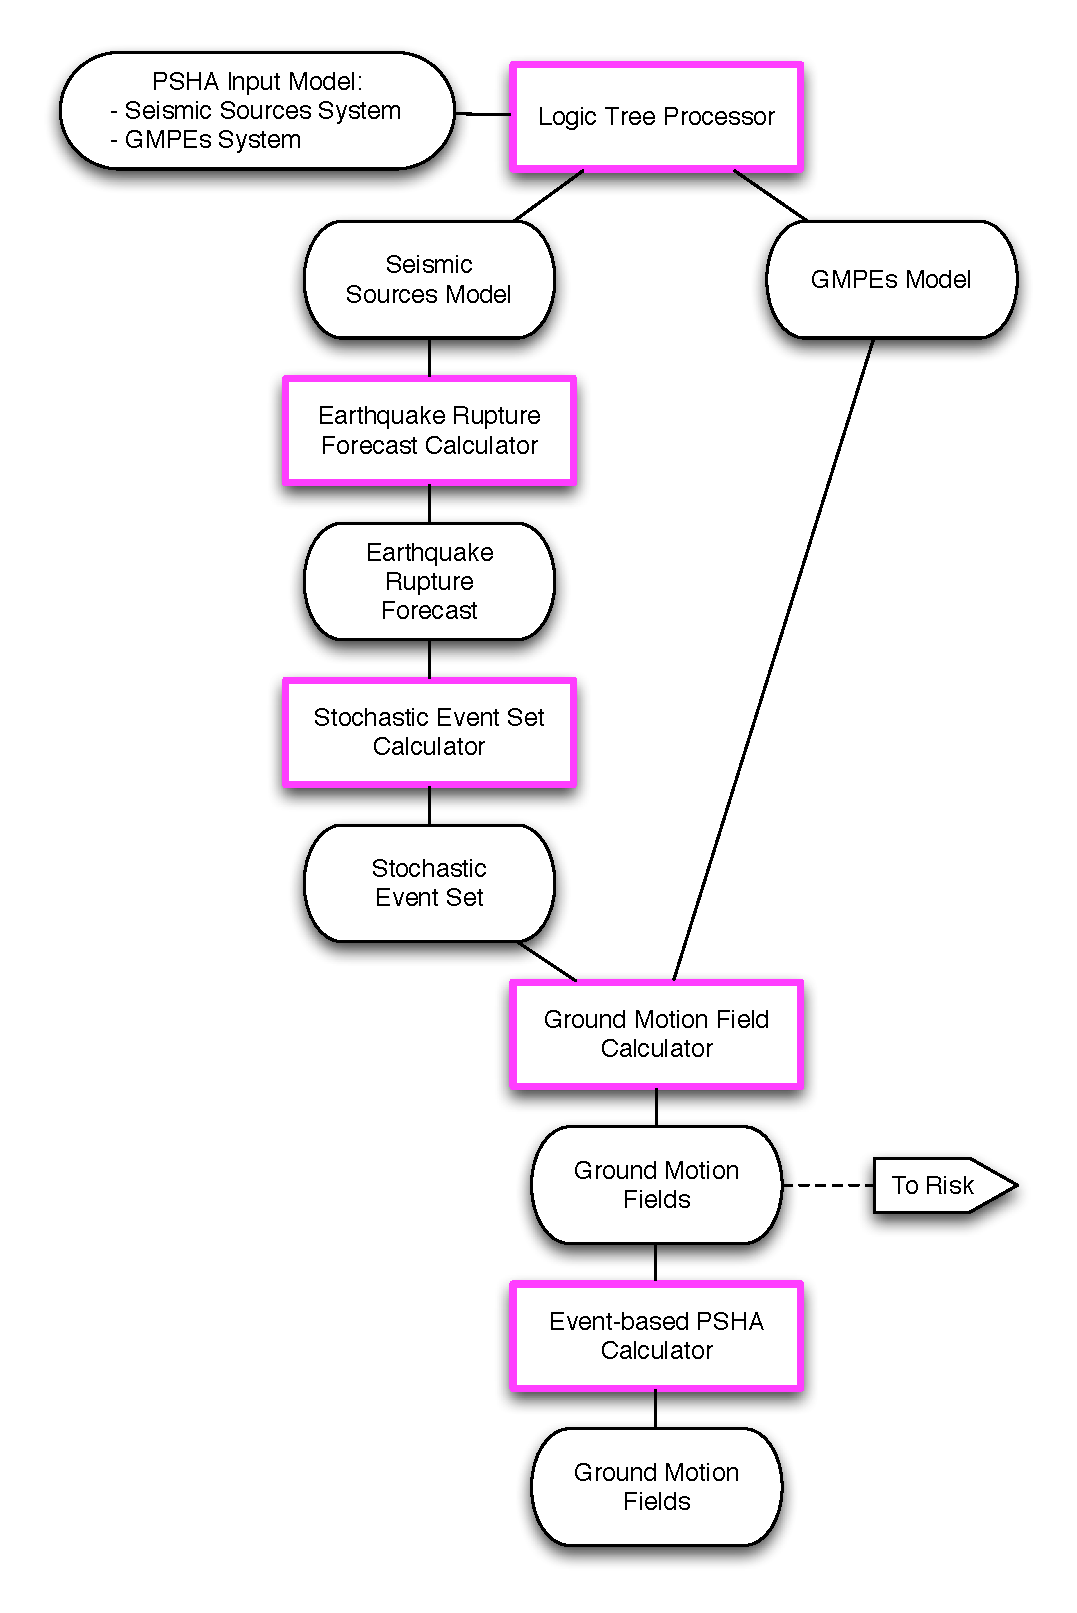
\includegraphics[width=7cm]{./Figures/Part_Hazard/event_based_workflow.eps}
\caption{Workflow for event-based PSHA. Similarly to the classical PSHA workflow (Figure \ref{classical_psha_workflow}), an ERF is computed, which is then used to generate a stochastic event set (representative of the seismic activity of a region in a given time span). Each event is then utilized to calculate a ground motion field over a region of interest.}
\label{event_based_workflow}
\end{center}
\end{figure}
\begin{figure}[htbp]
\begin{center}
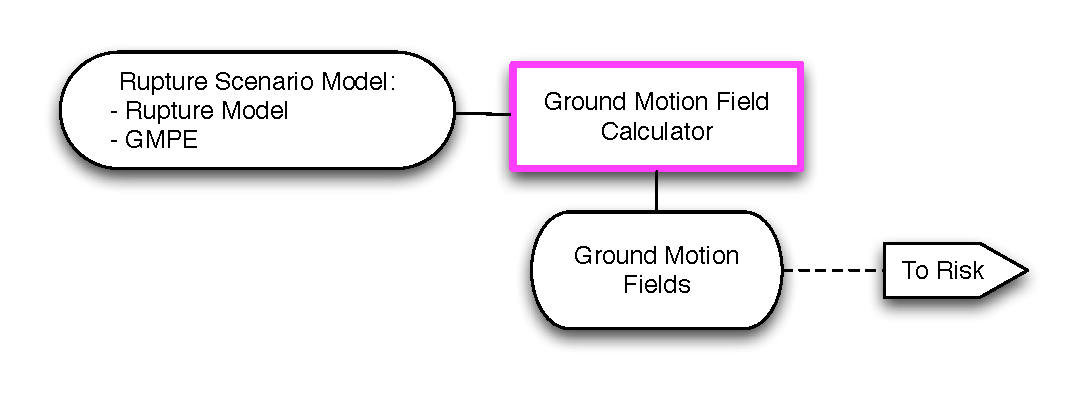
\includegraphics[width=7cm]{./Figures/Part_Hazard/deterministic_workflow.eps}
\caption{Workflow for deterministic SHA. Given a rupture scenario model, consisting of an earthquake rupture model, plus a GMPE, the ground motion field calculator can compute multiple ground motion field realizations (by taking into account GMPE aleatory uncertainties).}
\label{deterministic_workflow}
\end{center}
\end{figure}

